
\def\kt{\ensuremath{k_t}}
\newcommand{\Pmax}{p}
\newcommand{\CCFM}{CCFMa,CCFMb,Catani:1989sg,CCFMd}


%The proton PDFs are classically extracted from QCD fits by a measure of 
%the agreement between experimental data and corresponding theory models.
%During the fit procedure in the \fitter\ framework, the PDFs are
%parametrised at a starting scale $Q^2_0$ chosen to be below the charm 
%mass threshold and then evolved using coupled, integro-differential
%Dokshitzer-Gribov-Lipatov-Altarelli-Parisi 
%(DGLAP)~\cite{Gribov:1972ri,Gribov:1972rt,Lipatov:1974qm,
%Dokshitzer:1977sg,Altarelli:1977zs} evolution equations 
%as implemented in the QCDNUM~\cite{qcdnum} program in the $\overline{\text{MS}}$ scheme. 
%The evolution can be performed in the LO, NLO or NNLO accuracy~\cite{Curci:1980uw,Furmanski:1980cm}.
%
%In following, the theoretical models for various processes available in \fitter\ are described.
The PDFs are determined by measuring 
the agreement between experimental data and corresponding theory models. 
Models which are available in \fitter\ for various processes are described in the following text.


\subsection{Deep Inelastic Scattering Formalism and Schemes}
\label{dissection}


DIS data provide the tightest constraints on the PDFs so far.
Deep inelastic scattering is the lepton scattering on the 
constituents of the proton by a virtual exchange of a neutral (NC) 
or charged (CC) boson and, as a result, a scattered lepton and a 
multihadronic final state are produced.
The DIS kinematic variables are the negative squared four-momentum of 
the exchange boson, $Q^2$, the 
scaling variable $x$, which can be related in the parton model to 
the fraction of momentum carried by the struck quark, and the 
inelasticity parameter $y$, which is the fraction of the energy 
transferred to the hadronic vertex. 
\\
%
The NC (and similarly CC) cross section can be expressed in terms of structure functions:
\begin{eqnarray}
%  \nonumber
   \frac{d^2\sigma_{NC}^{e^{\pm} p}}{dxdQ^2}=\frac{2\pi\alpha^2}{xQ^4} 
     \big [ Y_{+} \tilde F_2^{\pm} \mp Y_{-}x \tilde F_3^{\pm} - y^2 \tilde F_L^{\pm} \big ],
 %\label{eq:NC not reduced}
\end{eqnarray}
where $Y_{\pm} = 1 \pm (1-y)^2$ with $y$ being the inelasticity. The structure function $\tilde F_2$
is the dominant contribution to the cross section, $x \tilde F_3$ is important at high $Q^2$ and $\tilde F_L$ is sizable 
only at high $y$. 
In the framework of perturbative QCD the structure functions are directly related to the 
parton distribution functions, i.e. in leading order (LO)  $F_2$ is the momentum sum of quark and anti-quark distributions, 
$F_2 \approx x \sum e^2_q (q+ \overline q)$, and $xF_3$ is related to their difference, 
    $xF_3 \approx x \sum 2e_q a_q (q- \overline q)$. At higher orders, terms related to the gluon density distribution
($\alpha_s g$) appear.
\\
In analogy to neutral currents, the inclusive CC $ep$ cross section can be expressed 
in terms of structure functions and in LO the $e^+p$ and $e^-p$ cross sections are sensitive to different quark 
densities:
\begin{eqnarray}
%  \nonumber
    \begin{array}{rll}
   e^{+}:  & & \tilde \sigma_{CC}^{e^{+} p} = 
                x[\overline u +\overline c] + (1-y)^2 x[ d+s ]  \\
   e^{-}:  & & \tilde \sigma_{CC}^{e^{-} p} = 
                x[ u +c] + (1-y)^2 x[\overline d +\overline s ].
    \end{array}
\end{eqnarray}
%
The QCD predictions for the DIS structure functions are obtained by convoluting 
the PDFs with the coefficient functions calculated using various schemes, i.e.
the general mass Variable-Flavour number (GM-VFN)~\cite{VFN} schemes or the
Fixed-Flavour number (FFN)~\cite{Laenen:1992, Laenen:1993, Riem:1995}, 
%\fitter\ implements the zero mass variable flavour number (ZMVFN) scheme
% from QCDNUM and are discussed in the following subsections.
%In the FFN scheme, heavy quark contributions are explicitly included in the 
%hard cross sections, . 
%In the VFN scheme, PDFs corresponding to heavy quarks are introduced and the number of active 
%flavors changes by one unit when the scale crosses the threshold for heavy quark distribution ($Q^2 > m_{Q}^2$).
%The various treatments for the heavy quark thresholds are implemented as provided by the MSTW group
%
%The evolution program QCDNUM~\cite{qcdnum} used in \fitter\ provides 
%the calculations of the deep inelastic structure functions in the zero-mass, 
%generalised mass and the fixed flavour number schemes. 
The following VFN schemes with various treatments for the heavy 
quark thresholds are considered in \fitter\ :
The Thorne Roberts (TR) scheme with its variants at NLO and
NNLO~\cite{Thorne:1997ga,Thorne:2006qt} as provided by the MSTW group,
the ACOT scheme with its variants at LO and NLO as provided by the CTEQ group. 
In addition, the zero-mass variable flavour number scheme (ZM-VFNS) where 
heavy quark densities are included in the proton for $Q^2>>m_h^2$ but are treated 
as massless in both the initial and final states can be used in \fitter\ .
The FFN scheme is available via the QCDNUM implementation and via the 
{\tt OPENQCDRAD}~\cite{openqcdrad:page} interface.
Each of these schemes is briefly discussed below.

\begin{description}
\item \bf {GM-VFN Thorne-Roberts scheme:} \rm
%\subsubsection{GM-VFN Thorne-Roberts scheme}
%
The Thorne-Roberts (TR) scheme smoothly connect the two regions: 
scales below ($Q^2<m_h^2$) and scales much above the heavy quark scale threshold ($Q^2>>m_h^2$). 
%However, the connection is not unique.
%A GM-VFNS can be defined by demanding equivalence of the $n_f = n$ (FFNS) 
%and $n_f = n+1$ flavour (ZM-VFNS) descriptions above the transition point for the new parton distributions
%(they are by definition identical below this point), at all orders.
There are two different variants of the TR schemes: TR standard (as used in MSTW PDF 
sets~\cite{Thorne:2006qt,Martin:epC63}) 
and TR optimal~\cite{Thorne:6180}, with a smoother transition across the heavy quark mass scales 
and both of them are accessible within the \fitter\ package.
The calculations are available to NLO and NNLO. In addition, a fast version of the scheme 
is available (i.e. RT FAST) by using the $k-factor$ technique where $k-factors$ are defined 
as the ratio between massless (accessed by QCDNUM) and massive scheme. 
The $k-factors$ are only calculated for the PDF parameters at the first fit iteration
hence, the recommended is the full TR scheme.
%Hence the RT-fast calculation must be repeated by inputting the final PDF parameters 
%and iterating this procedure until the input and output PDFs are not significantly different
%%%%
\vspace{0.1cm}
\item \bf {GM-VFN ACOT scheme:} \rm

The Aivazis-Collins-Olness-Tung scheme belongs to the group of VFN 
factorisation schemes that use the renormalization method of 
Collins-Wilczek-Zee (CWZ) \cite{CWZ}.
This scheme involves a mixture of the $\overline{\text{MS}}$ scheme 
for light and heavy (when the factorisation scale is larger than the heavy quark mass) partons
and the zero-momentum subtraction renormalisation scheme for graphs with heavy quark lines 
(if the factorisation scale is smaller than the mass of the heavy quark threshold). 
% is this sentence below is important?
%The DGLAP kernels and PDF evolution are pure $\overline{\text{MS}}$, 
%therefore, the ACOT scheme is considered to be a minimal extension of the $\overline{\text{MS}}$ scheme.

Within the ACOT package, different variants of the ACOT scheme are available:
ACOT-Full, S-ACOT-$\chi$, ACOT-ZM, $\overline{\text{MS}}$ at LO and NLO. 
For the longitudinal structure function higher order calculations are also available. 
The ACOT-Full implementation takes into account the quark masses 
and it reduces to ZM $\overline{\text{MS}}$ scheme in the limit of masses going to zero, 
but it has the disadvantage of being quite slow.
Therefore the $k-factor$ technique has been adopted within the \fitter\ framework which are  
defined in two different ways:
as the ratio between same order calculations but massless vs massive 
(i.e. NLO (ZM-VFNS)/NLO (ACOT), or as the ratio between LO (massless)/NLO (massive),
both giving similar results.
%%For convergence of the k-factors usually $2-3$ repetitions of the fit are needed.
%
%The different variants of this scheme are all integrated in the \fitter\  framework and can be 
%selected via the namelist {\tt HF$\_$SCHEME} in the {\tt steering.txt} (ACOT ZM, ACOT FULL, S-ACOT Chi).
%
%The differences between TR and ACOT scheme types are summarised in the figure \ref{fig:schemes}.
%One major issue in a complete GM-VFNS, is that of the ordering of the
%perturbative expansion.
%The equivalency of swapping the $O(m_{H}^2/Q^2)$ terms between Wilson coefficients (or hard-scattering amplitudes) 
%without violating the definition of a GM-VFNS is what mainly distinguish the ACOT from TR schemes. 
%
%In ACOT, the massive result is included up to O(alpha_s),
%in TR, it is attempted to included it up to O(alpha_s^2).
%%%%
\vspace{0.1cm}
\item \bf {Fixed-Flavour Number Scheme:} \rm

In the FFN scheme only the gluon and the light quarks are considered
as partons within the proton and massive quarks are produced perturbatively in the final state.
In \fitter\ this scheme can be accessed via the 
QCDNUM implementation or interface to the open-source code OPENQCDRAD (ABM)~\cite{openqcdrad:page}.
The later implementation also includes the running mass definition of the heavy quark 
mass ~\cite{Alekhin:runm}.
This scheme has the advantage of reducing the sensitivity of the DIS cross sections to
higher order corrections, and improving the theoretical precision of the mass definition. 
In QCDNUM, the calculation of the heavy quark contributions to DIS structure functions
are available at NLO and only electromagnetic exchange contributions are taken into account.
In the ABM implementation, the QCD corrections to the massive Wilson coefficients 
up to the currently best known approximate NNLO for the NC heavy-quark 
production~\cite{SMoch:npb864} and up to NLO for the CC case are available.
\end{description}

%%%%%%%%%%%
%\item \bf {Electroweak corrections for \texorpdfstring{$ep$}{ep} scattering:} \rm
The calculations of higher-order electroweak corrections to DIS scattering at 
HERA are performed in the on-shell scheme where the gauge bosons masses $M_W$ and 
$M_Z$ are treated symmetrically as basic parameters together with the top, Higgs 
and fermion masses.
\\
In the \fitter\, the electroweak corrections 
for the DIS process are based on the EPRC package~\cite{SpiesbergerPrivComm}.
The code provides the running of $\alpha$ using the most recent parametrisation
of the hadronic contribution to $\Delta_\alpha$ \cite{Jegerlehner}, as well as 
an older one from Burkhard \cite{Burkhard}.


\subsection{Diffractive PDFs}

\newcommand{\asotp}{\ensuremath{\frac{\alpha_{\rm s}}{2\pi}}}
\newcommand{\Sgl}[1]{\ensuremath{\tilde f_{#1+}}}
\newcommand{\Pom}{{I\!P}}
\newcommand{\Reg}{{I\!R}}
\newcommand{\xpom}{$x_{I\!P}$}


Similar to standard DIS, diffractive parton distributions (DPDFs) 
can be derived from QCD fits to diffractive cross sections.
%In this section the diffractive process is briefly described.
At HERA about 10\% of deep inelastic interactions are diffractive leading to
events in which the interacting proton stays intact ($ep\to eXp$). 
In the diffractive process the proton appears well separated from the 
rest of the hadronic final state by a large rapidity gap  
and is interpreted as the diffractive dissociation 
of the exchanged virtual photon to produce a hadronic system $X$ with mass much 
smaller than $W$ and the same net quantum numbers as the exchanged photon.
%Figure~\ref{fig:diff} illustrates the kinematic variables used to describe
%the inclusive diffractive DIS process. 
For such process, the proton vertex factorisation approach
is assumed where the diffractive DIS is mediated by the exchange of hard Pomeron and a
secondary Reggeon. 
The factorisable pomeron picture has proved remarkably successful for the description of most of these data.
%
%\begin{figure}[!ht]
%\begin{center}
%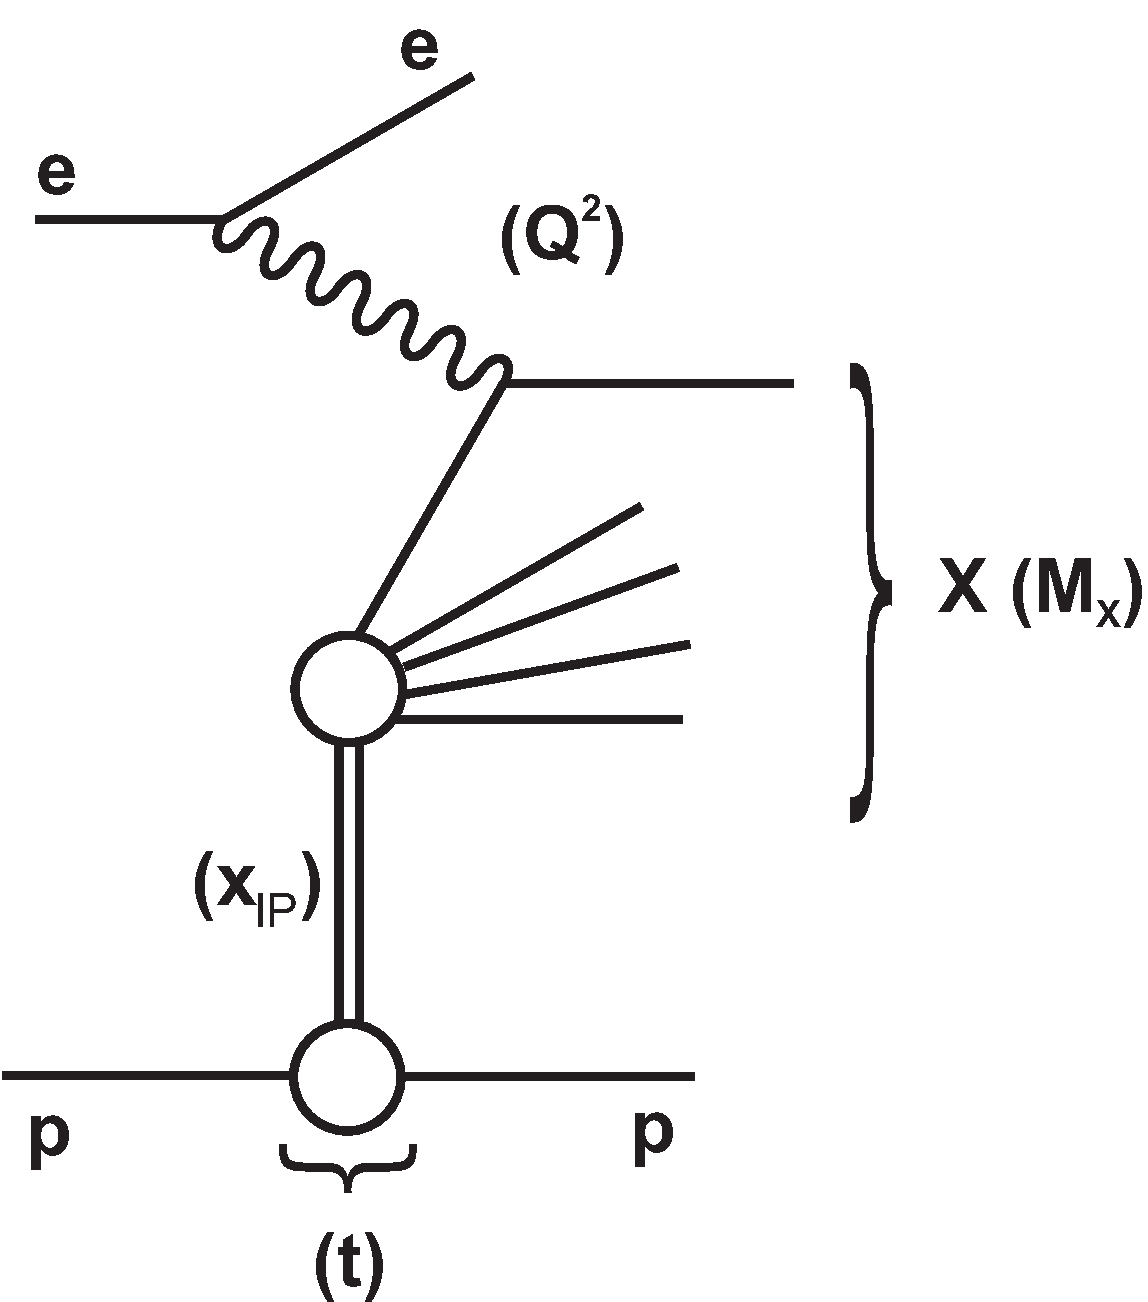
\includegraphics[width=0.5\linewidth]{figures/diffraction.pdf}
%\end{center}
%\caption{Schematic diagram of the kinematic variables used to
% describe the inclusive diffractive DIS process.}
%\label{fig:diff}
%\end{figure}

In addition to $x$, $Q^2$ and the squared four-momentum transfer $t$
(the undetected momentum transfer to the proton system),
the mass $M_X$ of the diffractively produced final state provides
 a further degree of freedom. In practice, the variable $M_X$ 
is often replaced by $\beta=\frac{Q^2}{M_X^2+Q^2-t}$.
%
In models based on a factorisable pomeron, $\beta$ may be viewed as the fraction of the
pomeron longitudinal momentum which is carried by the struck parton, $x=\beta x_{\Pom}$.
%The diffractive parton distribution functions (DPDFs) are interpreted as probabilities for 
%finding a parton with a small fraction of the proton momentum $x=\beta\Pom$

For the inclusive case, the diffractive cross-section can be expressed as:
\begin{equation}
\begin{array}{lcl}
  \frac{d\sigma}{d\beta\,dQ^2dx_{\Pom}\,dt}
=
  \frac{2\pi\alpha^2}{\beta Q^4}\,
    \left( 1 +  (1-y)^2 \right) \ensuremath{\overline\sigma}^{D(4)}(\beta,Q^2,x_{\Pom},t)
\label{Dxs}
\end{array}
\end{equation}
where the ``reduced cross-section'' , $\overline\sigma$, is defined as
\begin{equation}
\begin{array}{lcl}
\overline\sigma^{D(4)}
 = F_2^{D(4)} - \frac{y^2}{1 +  (1-y)^2}\, F_L^{D(4)}
 = F_T^{D(4)} + \frac{2(1-y)}{1 +  (1-y)^2}\, F_L^{D(4)}.
\label{eq:sigred}
\end{array}
\end{equation}
%The dimension of $F_k^{D(4)}(\beta,Q^2,x_{\Pom},t)$
%is $GeV^{-2}$ and thus quantities integrated over $t$.
%\begin{equation}
%F_k^{D(3)}(\beta,Q^2,x_{\Pom})
%\equiv
%\int_{t_{\rm min}}^{t_{\rm max}} dt
%F_k^{D(4)}(\beta,Q^2,x_{\Pom},t)
%\end{equation}
%are dimensionless. The maximum kinematically allowed value of $t$ is given by
%\begin{equation}
%t_{\rm MAX} 
%=
%-\frac{x_{\Pom}^2 m_p^2 + p_\perp^2}{1-x_{\Pom}}
%\approx 
%-\frac{x_{\Pom}^2}{1-x_{\Pom}} m_p^2
%\end{equation}
%where $m_p$ is the proton mass.
With $x = x_{\Pom}\beta$ we can normalize to the standard DIS formula.
%\begin{equation}
%\begin{array}{lcl}
%\frac{d\sigma}{d\beta\,dQ^2\,dx_{\Pom}\,dt} =
%  \frac{2\pi\alpha^2}{x\, Q^4}\,
%    \left( 1 +  (1-y)^2 \right) x_{\Pom}\ensuremath{\overline\sigma}^{D(4)}(\beta,Q^2,x_{\Pom},t)
%\end{array}
%\end{equation}
%which upon integration over $t$ reads
%\begin{equation}
%\begin{array}{lcl}
%\label{Dxs3}
%  \frac{d\sigma}{d\beta\,dQ^2\,dx_{\Pom}}
%=  
%  \frac{2\pi\alpha^2}{x Q^4}\,
%    \left( 1 +  (1-y)^2 \right) \,x_{\Pom}\ensuremath{\overline\sigma}^{D(3)}(\beta,Q^2,x_{\Pom}).
%\end{array}
%\end{equation}
%%The H1 and ZEUS data files typically contain $x_{\Pom}\ensuremath{\overline\sigma}^{D(3)}$.
The diffractive structure functions can be expressed as convolutions of the
calculable coefficient functions with diffractive quark and gluon distribution functions,
 which in general depend on all of \xpom, $Q^2$, $\beta$, $t$.
\\
\\
%==========================================
%{\bf Regge factorization} 
%Needed? \\
The diffractive PDFs in \fitter are implemented following the prescription of ZEUS
publication~\cite{zeus:diff2009} and can be used to reproduce the main results.
%For a  better description of data, a contribution from a secondary Reggeon, $\Reg$, is included, hence
%\begin{equation}
%F_k^{D(4)}(\beta,Q^2,x_{\Pom},t) = 
%\sum_{\mathcal{X} =\Pom,\Reg}
%\phi_\mathcal{X}(x_{\Pom},t)\, F^\mathcal{X}_k(\beta,Q^2)
%\end{equation}
%or
%\begin{equation}
%\label{eq:FD3}
%F_k^{D(3)}(\beta,Q^2,x_{\Pom}) = 
%\sum_{\mathcal{X} =\Pom,\Reg}
%\Phi_\mathcal{X}(x_{\Pom})\, F^\mathcal{X}_k(\beta,Q^2)
%\end{equation}
%where
%\begin{equation}
%\label{eq:intFlux}
%\Phi_{\mathcal{X}}(x_{\Pom}) =
%\int\limits_{t_{\rm min}}^{t_{\rm max}} dt\, \phi_\mathcal{X}(x_{\Pom},t)
%\,.
%\end{equation}
%The fluxes are parametrized as
%\begin{subequations}
%\label{eq:flux}
%\begin{equation}
%\phi_\mathcal{X}(x_{\Pom},t) = 
%\frac {A_\mathcal{X}\, e^{b_\mathcal{X} t}} {x_{\Pom}^{2\alpha_\mathcal{X}(t) -1}}
%\end{equation}
%where
%\begin{equation}
%\alpha_\mathcal{X}(t) = \alpha_\mathcal{X}(0) + \alpha_\mathcal{X}' t
%\,.
%\end{equation}
%\end{subequations}
%The function $F^\Reg_k(\beta,Q^2)$  is taken to be that of the pion.
%
\subsection{Alternative to DGLAP DIS models}
Different approaches that are alternative to DGLAP formalism can be used to analyse DIS data in \fitter .
Those include several dipole models and transverse momentum dependent, or unintegrated PDFs, uPDFs.
Both approaches are discussed below.

\subsubsection{DIPOLE models}

The dipole picture provides an alternative approach to the virtual photon-proton
 scattering at low $x$  because it allows the description of both inclusive and 
diffractive processes.
 In this approach, the virtual photon fluctuates into a $q\bar q$ (or $q\bar q g$) 
 dipole which interacts with the proton~\cite{NNZ:91}.  
The dipoles can be viewed as quasi-stable quantum mechanical states, which have very long 
life time $\propto 1/m_p x\;$ and a size which is not changed by scattering.
%A schematic view of dipole factorisation at small $x$ in DIS is illustrated in figure~\ref{fig:dipole}.
The virtual photon fluctuates into a quark-antiquark pair and subsequently interacts with the target, 
and the dynamics of the interaction are embedded in the dipole scattering amplitude.

%\begin{figure}
%\begin{center}
%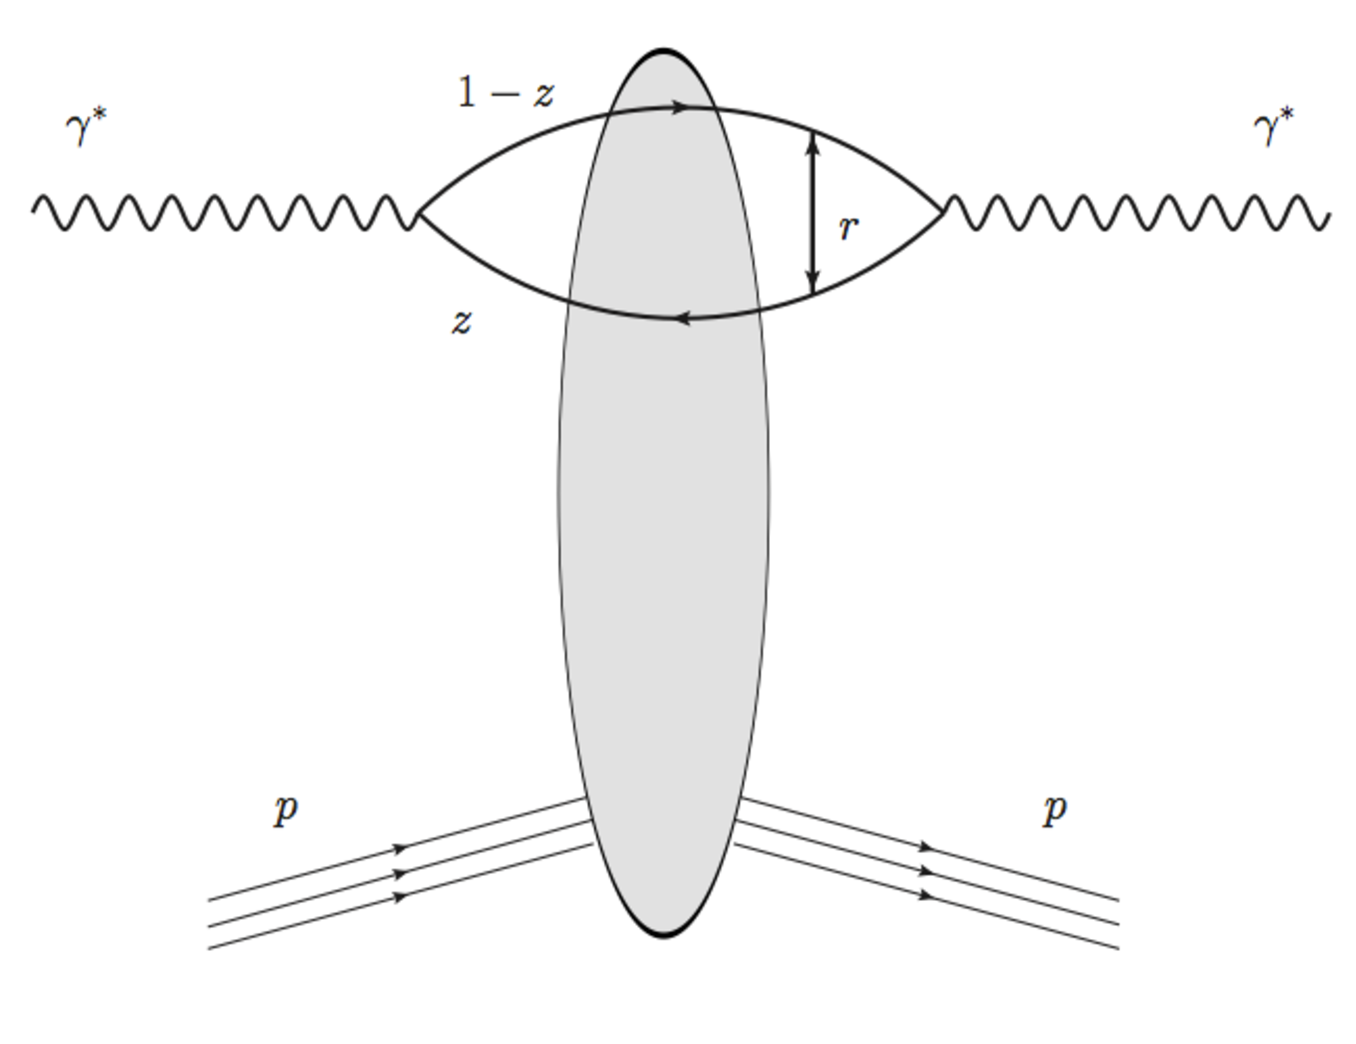
\includegraphics[width=0.5\linewidth]{figures/dipole.pdf}
%\end{center}
%\caption{Schematic diagram of dipole factorisation for the inclusive cross section in DIS.}
%\label{fig:dipole}
%\end{figure}

Several dipole models which assume different behavior of the dipole-proton 
cross sections are implemented in \fitter\ :
%\begin{itemize}
%\item the original Golec-Biernat-W\"usthoff (GBW)~\cite{Golec-Biernat:1998js} 
the Golec-Biernat-W\"usthoff (GBW)
dipole saturation model~\cite{Golec-Biernat:1998js},
the colour glass condensate approach to the high parton density 
regime Iancu-Itakura-Munier (IIM) model~\cite{Iancu:2003ge} and 
a modified GBW model which takes into account the effects of  
DGLAP evolution Bartels-Golec-Kowalski (BGK)~\cite{Bartels:2002cj}.
%\end{itemize}

\begin{description}
\item \bf {GBW model:} \rm
In the GBW model the dipole-proton cross section $\sigma_{\text{dip}}$ is given by
\begin{equation}
\label{eGBW}
   \sigma_{\text{dip}}(x,r^{2}) = \sigma_{0} \left(1 - \exp \left[-\frac{r^{2}}{4R_{0}^{2}(x)} \right]\right),
\end{equation}
here $r$ corresponds to the transverse separation between the quark and the antiquark, and $R_{0}^{2}$
 is 
%an $x$ dependent scale parameter, having the form $R_{0}^{2}(x)=\left(x/x_{0}\right)^{\lambda}$.
an $x$ dependent scale parameter which has corresponds to a saturation radius,  $R_{0}^{2}(x)=\left(x/x_{0}\right)^{\lambda}$.
The free fitted parameters are the cross-section normalisation $\sigma_{0}$ as well as $x_{0}$ and $\lambda$.
%%%%

\vspace{0.1cm}
\item \bf {IIM model:} \rm
The IIM model assumes an improved expression for the dipole cross section which is based on the 
Balitsky-Kovchegov equation~\cite{Balitsky:1995ub}. The explicit formula for $\sigma_{\text{dip}}$ 
can be found in~\cite{Iancu:2003ge}. The free fitted parameters are an alternative scale parameter $\tilde{R}$, $x_{0}$ and $\lambda$.
%%%%

\vspace{0.1cm}
\item \bf {BGK model:} \rm
The BGK model modifies the GBW model by taking into account the  DGLAP evolution
of the gluon density. 
The dipole cross section is given by
\begin{equation}
\begin{array}{lcl}
   \sigma_{\text{dip}}(x,r^{2})  =  \sigma_{0} 
\left(1 - \exp \left[-\frac{\pi^{2} r^{2} \alpha_{s}(\mu^{2}) xg(x,\mu^{2})}{3 \sigma_{0}} \right]\right).
\end{array}
\label{eBGK}
\end{equation}
The factorization scale $\mu^{2}$ has the form $\mu^{2} = C_{bgk}/r^{2}+\mu^{2}_{0}$.
%This model uses the following gluon density at the starting scale $Q_{0}^{2}=1\mbox{ GeV}^{2}$
In this model the gluon density parametrized at some starting scale $Q_{0}^{2}$ by
$ xg(x) = A_{g} x^{-\lambda_{g}}(1-x)^{C_{g}} $
is evolved to larger scales using LO and NLO DGLAP evolution.
The free fitted parameters for this model are $\sigma_{0}$, $\mu^{2}_{0}$ and three parameters for the gluon density: $A_{g}$, $\lambda_{g}$, $C_{g}$. The parameter $C_{bgk}$ is kept fixed: $C_{bgk} = 4.0$. 
%%%%

\vspace{0.1cm}
\item \bf {BGK model with valence quarks:} \rm

The dipole models are valid in the low-$x$ region only, where the valence quark contribution is small, of the order of 5\%. The new HERA $F_2$ data have a precision which is  better than 2 \%. Therefore, in the \fitter\ the contribution of the valence quarks is taken from the PDF fits and added to the original 
BGK model, this is uniquely possible within the \fitter\ framework.
% The quality of the fits of the BGK dipole model with valence quarks and without 
%valence quarks are the same.
\end{description}

\subsubsection{Transverse Momentum Dependent (unintegrated PDF) with CCFM}

Here another alternative approach to collinear DGLAP evolution is presented.
In high energy factorization \cite{Catani:1990eg} the measured cross section is written
 as a convolution of the partonic cross section $\hat{\sigma}(É \kt),$ which depends on the transverse 
momentum $\kt$ of the incoming parton, with the $\kt$-dependent parton distribution function 
${\cal \tilde A}\left(x,\kt,\Pmax\right)$ (transverse momentum dependent (TMD) or unintegrated uPDF):
\begin{equation}
 \sigma  = \int 
\frac{dz}{z} d^2k_t \hat{\sigma}(\frac{x}{z},k_t)  {\cal \tilde A}\left(x,\kt,\Pmax\right)
\label{kt-factorisation}
\end{equation}
Generally, the evolution of ${\cal \tilde A}\left(x,\kt,\Pmax\right)$ 
can proceed via the BFKL, DGLAP or via the CCFM evolution equations.
In \fitter\, an extension of the CCFM~\cite{\CCFM} evolution has been implemented.
Since the evolution cannot be easily obtained in  a closed form, 
 first a kernel $ {\cal \tilde A}\left(x'',\kt,\Pmax\right) $ 
is determined from the MC solution of the CCFM evolution equation, 
and is then folded with the non-perturbative starting distribution 
${\cal A}_0 (x)$~\cite{Jung:2012hy}:
\begin{eqnarray}
%\begin{align}
 x {\cal A}(x,\kt,\Pmax) & = & 
   x\int dx' \int dx'' {\cal A}_0 (x) {\cal \tilde A}\left(x'',\kt,\Pmax\right)  \delta(x' \cdot x'' - x) \nonumber \\  
 & = & \int dx' \int dx'' {\cal A}_0 (x) {\cal \tilde A}\left(x'',\kt,\Pmax\right) \frac{x}{x'} \delta(x'' - \frac{x}{x'}) \nonumber \\ 
 & = & \int dx' {{\cal A}_0 (x') }  \cdot \frac{x}{x'}{ {\cal \tilde A}\left(\frac{x}{x'},\kt,\Pmax\right). } 
%\end{align}
\end{eqnarray}
%An intrinsic $\kt$ dependence is included in the kernel ${\cal \tilde A}$
%\begin{eqnarray}
%{\cal \tilde A} & = & {\cal \tilde A'} \cdot f(k_{t\;0}) = {\cal \tilde A'} \cdot  \exp\left[ 
%-\frac{(\mu-k_{t\;0})^2}{\sigma^2}\right]
%\end{eqnarray}
The kernel  ${\cal \tilde A}$ includes all the dynamics of the evolution,
 Sudakov form factors and splitting functions and is determined in 
a grid of $50\otimes50\otimes50$ bins in $x,\kt,\Pmax$.  

The calculation of the cross section according to Eq.(\ref{kt-factorisation})
 involves a multidimensional Monte Carlo integration which is time consuming
 and suffers from numerical fluctuations, and therefore cannot be used directly in a fit
 procedure.
% involving the calculation of numerical derivatives in the search for a minimum. 
Instead the following procedure is applied:
\begin{eqnarray}
\nonumber
\sigma_r(x,Q^2) & = & \int_x^1 d x_g {\cal A}(x_g,\kt,\Pmax) \hat{ \sigma}(x,x_g,Q^2) \\
  & = & \int_x^1 dx' {\cal A}_0 (x') \cdot \tilde{ \sigma}(x/x',Q^2). 
  \label{final-convolution}
\end{eqnarray}

The kernel ${\cal \tilde A}$ has to be provided separately and is not
 calculable within the program. A starting distribution  ${\cal A}_0$, 
 at the starting scale $Q_0$, of the following form is used:
\begin{eqnarray}
x{\cal A}_0(x,\kt) &=& N x^{-B_g} \cdot (1 -x)^{C_g}\left( 1 -D_g x\right) 
\label{a0}
\end{eqnarray}
with free parameters $N,\, B_g,\, C_g,\, D_g$. 
%In the present version, only the transverse momentum dependent gluon distribution 
%can be obtained from the fit. 

The calculation of the $ep$ cross section follows eq.(\ref{kt-factorisation}), 
with the off-shell matrix element including quarks masses taken from \cite{Catani:1990eg} 
in its implementation in {\tt CASCADE} \cite{Jung:2010si}.
In addition to the boson gluon fusion process, valence quark initiated 
$\gamma q\to q$ processes are also included, with the valence quarks taken from~\cite{Deak:2010gk}.


\subsection{Drell Yan processes}
\label{dysection}

%This section presents calculations of Drell Yan processes that can be used to 
%predict lepton pair production at the LHC or Tevatron.
The Drell Yan (DY) process constrain all different quark combinations
providing valuable information about PDFs.
%
Presently, the calculations of the DY processes are known for many observables up to 
NNLO order, for example, MCFM~\cite{MCFM} package is available for NLO calculations,
FEWZ~\cite{FEWZ} and DYNNLO~\cite{DYNNLO} for NLO and NNLO. Due to the complicated 
nature of these calculation involving an increased number of diagrams with each 
additional order, they are too slow to be used iteratively in a fit.
There are several methods available to speed-up such calculations two of which 
are implemented into \fitter\ : the $k-factor$ approximation from lower (LO) to higher order (NLO) 
and the so-called grid technique using an interface to the APPLGRID, both of them shortly
described below.  
%(storing the matrix elements on grids such that the cross sections maybe 
% calculated later by convoluting these grids with the input PDFs) when available.
%\begin{figure}[!ht]
%\begin{center}
%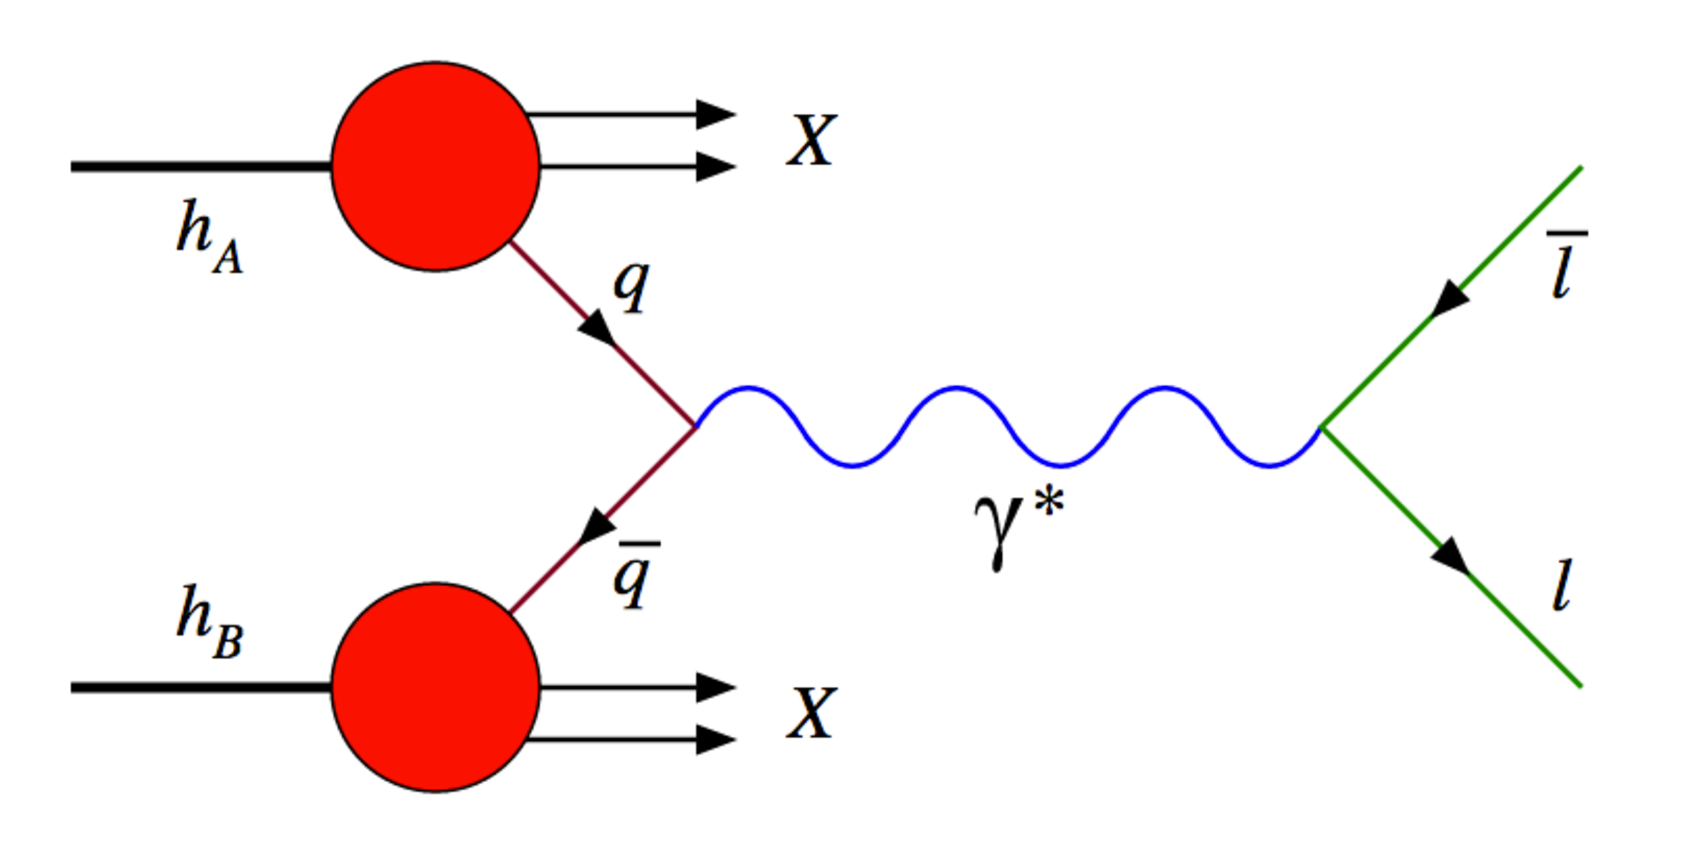
\includegraphics[width=0.5\linewidth]{figures/dy.pdf}
%\end{center}
%\caption{Diagram for a generic DY scattering.}
%\label{fig:dy}
%\end{figure}
 % 
%\fitter\ provides two implementations for $pp$  Drell Yan processes.
%The first implementation uses calculations at LO which can be extended to NLO using k-factors,
%the second uses the APPLGRID interface. 

\begin{description}
\item \bf {$k-factor$ technique:} \rm
The leading order DY triple differential cross section in
invariant mass \(M\), boson rapidity \(y\) and CMS
lepton scattering angle \(\cos\theta\), for the neutral current, 
can be written as~\cite{Drell:1970wh,Yamada:1981mw}:
\begin{align}
% \scriptstyle
 \textstyle
% \frac{\mathrm{d}^3\sigma}{\mathrm{d}M\mathrm{d}y\mathrm{d}\cos\theta} &= 
 \frac{d^3\sigma}{dM{d}y d\cos\theta} =  
 \frac{\pi\alpha^2}{3MS}\sum_{q}P_q \left[F_q(x_1,Q^2)F_{\bar{q}}(x_2,Q^2) 
 + (q\leftrightarrow\bar{q})\right],
\end{align}
where \(S\) is the squared CMS beam energy, \(x_{1,2} = \frac{M}{\sqrt{S}}\exp(\pm y)\), $F_q(x_1,Q^2)$ 
is the parton number density, and 
\begin{align}
  P_q &=  e_l^2e_q^2(1+\cos^2\theta) \nonumber \\
      &+  e_le_q\frac{2M^2(M^2-M_Z^2)}{\sin^2\theta_W\cos^2\theta_W
          \big[(M^2-M_Z^2)^2+\Gamma_Z^2M_Z^2\big]} \nonumber \\
      &    \big[aA_q(1+\cos^2\theta)+2bB_q\cos\theta\big] \nonumber \\
      &+  \frac{M^4}{\sin^4\theta_W\cos^4\theta_W
          \big[(M^2-M_Z^2)^2+\Gamma_Z^2M_Z^2\big]} \nonumber \\
      &    \big[(a^2+b^2)(A_q^2+B_q^2)(1+\cos^2\theta)+8abA_qB_q\cos\theta\big].
\end{align}
Here \(\theta_W\) is the Weinberg angle, \(M_Z\) and \(\Gamma_Z\) are Z boson mass and 
width, $a, b, A_q, B_q, e_l, e_q$ are electro-weak couplings.
%\begin{align}
% a & = -\frac{1}{4} + \sin^2\theta_W, \  b  = -\frac{1}{4}, \nonumber \\
% A_q & = \frac{1}{2}I_q^3-e_q\sin^2\theta_W, \ B_q  = \frac{1}{2}I_q^3, \ I_u^3  = -I_d^3 = \frac{1}{2},  \nonumber \\
% e_l & = -1, e_u = \frac{2}{3}, e_d = -\frac{1}{3}.
%\end{align}
\\
\\
The expression for charged current scattering has a simpler form.
\begin{align}
\frac{d^3\sigma}{dMdyd\cos\theta} &=
 \frac{\pi\alpha^2}{48S\sin^4\theta_W}
 \frac{M^3(1-\cos\theta)^2}{(M^2-M_W^2)+\Gamma_W^2M_W^2}  \nonumber \\
 & \sum_{q_1,q_2}V_{q_1q_2}^2F_{q_1}(x_1,Q^2)F_{q_2}(x_2,Q^2),
\end{align}
where \(V_{q_1q_2}\) is the CKM quark mixing matrix and \(M_W\) and \(\Gamma_W\)
are \(W\) boson mass and decay width.

The simple form of these expressions allows the calculation of integrated
cross sections without utilization of Monte-Carlo techniques which often 
introduce statistical fluctuations.
%This is particularly useful for PDF fitting purposes because
%statistical fluctuations are avoided in this case. 
In both neutral and charged current expressions the parton distribution functions
factorise as functions dependent only on boson rapidity \(y\) and
invariant mass \(M\).
%leaving \(\cos\theta\) dependence aside.
The integral in \(\cos\theta\) can be computed analytically and
integrations in \(y\) and \(M\) can be performed with the Simpson
method. The \(\cos\theta\) parts are kept in the equation 
explicitly because their integration is asymmetric for
data in lepton \(\eta\) bins and also because of the need to apply 
lepton \(p_{\perp}\) cuts.

The fact that PDF functions factorise, allows high speed calculations when 
performing parameter fits over lepton rapidity data. In this case
the factorised part of the expression which is independent of PDFs can be
calculated only once for all minimisation iterations.
The leading order code in \fitter\ package implements this 
optimisation and uses fast convolution routines provided by
QCDNUM. Currently the full width LO calculations are optimised 
for lepton pseudorapidity and boson rapidity distributions with the
possibility to apply lepton \(p_{\perp}\) cuts.
%making this procedure flexible to describe data.
This flexibility allows the calculations to be performed within the phase space
corresponding to the available measurement.

%The calculated leading order cross sections are multiplied by
%NLO or NNLO k-factors provided for corresponding data distributions.
The calculated leading order cross sections are multiplied by
$k-factors$ to obtain predictions at NLO.
\\
%or NNLO precision.
%%%%
%\subsubsection{APPLGRID}
%\vspace{0.1cm}
\item \bf {APPLGRID technique:} \rm
The APPLGRID~\cite{Carli:2010rw} package allows the fast computation 
of NLO cross sections for particular processes for arbitrary sets of 
proton parton distribution functions. The package implements
calculations of DY production as well as jet production in $pp(\bar p)$
collisions and DIS processes. 

The approach is based on storing the perturbative coefficients
of NLO QCD calculations of final-state observables measured
in hadron colliders in look-up tables. The PDFs and the 
strong couplings are included during the final calculations,
e.g. during PDF fitting. The method allows 
variation of factorization and renormalization scales in
calculations.

The look-up tables (grids) can be generated with modified versions
of MCFM parton level generator~\cite{Campbell:1999ah,Campbell:2010ff} 
or NLOjet++~\cite{Nagy:2001fj} code for the jet production.
The model input parameters are in fact pre-set following the 
MCFM input steering card, while binning and definitions of the
cross section observables are set in the APPLGRID code.
%as distributed with the full version of APPLGRID package.
% NLO calculations
%for the current analysis are performed with the help of APPLGRID
%generated grids based on MCFM calculations. 
%
%APPLGRID supports an interface to the MCFM parton level generators,
%hence model input parameters such as electroweak parameters
%are in fact pre-set following the MCFM input steering card, while
%binning and definitions of the observables for which the
%differential cross sections are needed are set in the 
%APPLGRID code. 
%The grid parameters \(x_1, x_2\) and \(Q^2\) binning
The grid parameters, \(Q^2\) binning
and interpolation orders are also defined in the code.

APPLGRID constructs the grid tables in two 
steps: {\it (i)} exploration of the phase space in order
to optimize the memory storage and {\it (ii)} actual grid
construction in the phase space corresponding to the 
requested observables.
Afterwards the NLO cross sections are restored from the grids
using externally provided PDFs, \(\alpha_S\), factorization and 
renormalization scales. QCD NNLO $k-factors$ can be applied
if requested.

\end{description}

%Alternatively, one can obtain the NLO predictions directly by using 
%APPLGRID or FASTNLO techniques, which rely on the factorisation theorem by 
%decoupling the hard scattering coefficients from PDFs.
%The hard scattering coefficients are calculated once and stored into a grid 
%for a given kinematic bin, speeding up the convolution process with the PDFs 
%and thus allowing to for fast QCD fits. 


%These methods are described in more detail in section \ref{sec:theory:jets}.
%An independent treatment for the electro-weak corrections is applied as the 
%independent k-factors, using packages such as SANC and FEWZ.

\subsection{Cross Sections for \texorpdfstring{$t\bar{t}$}{t-tbar} production in $pp$ or $p\bar p$ collisions}
%This section presents the calculation tool available 
%in \fitter\ for top-guark pair prouction in $p \bar{p}$ and $pp$ collisions.
%
Top-quark pairs ($t\bar{t}$) are mainly produced at hadron colliders via $gg$ fusion and
$q \bar q$ annihilation thus providing possibility to constrain the gluon density in the proton. 
%There are also $q q'$ and $q g$ production modes.
In \fitter\ the program HATHOR~\cite{Aliev:2010zk} is interfaced which allows the calculation of 
the expected total $t \bar t$ cross section at 
$p \bar p$ and $p p$ colliders up to approximate NNLO accuracy.
Version 1.3 of HATHOR includes the exact NNLO for $q \bar q \to t \bar t$ \cite{Baernreuther:2012ws}
as well as a new high-energy constraint on the approximate NNLO calculation obtained from
soft-gluon resummation \cite{Moch:2012mk}.
The default choice for renormalization and factorization scale in $t \bar t$ production is the top-quark mass, $m_t$.
The pole mass scheme is typically employed for $m_t$ but HATHOR also supports calculations in
the $\overline{\text{MS}}$ scheme.

\subsection{Jet production}
\label{jetsection}
%In this subsection, the use of the factorisation formalism is fully exploited for the 
%calculations of the inclusive jets and dijet cross sections.
%This sections presents various fast calculational techniques for jet production based on
%the factorization formalism.

Similarly to DY case, the calculation of higher order jet cross sections 
is very demanding in terms of computing power. 
Therefore, in order to enable the inclusion of jet-cross section 
measurements in PDF and $\alpha_s$ fits, the perturbative
coefficients have to be pre-computed in a PDF and $\alpha_s$ 
independent way. For this purpose, two grid tools are
interfaced to the \fitter , APPLGRID (see~\ref{dysection}) and 
FastNLO.

\begin{description}
\item \bf {FastNLO technique:} \rm
The fastNLO project~\cite{Kluge:2006xs,Wobisch:2011ij,Britzger:2012bs}
%enables the inclusion of jet data in PDF and $\alpha_s$ fits.
uses multi-dimensional interpolation
techniques to convert the convolutions of perturbative 
coefficients with parton distribution functions and 
the strong coupling into simple products.
%Although the concept is process independent, 
The perturbative 
coefficients are calculated by the \texttt{NLOJET++}
program~\cite{Nagy:1998bb} where calculations for jet-production
in DIS~\cite{Nagy:2001xb}  as well as in hadron-hadron 
collisions~\cite{Nagy:2003tz,Nagy:2001fj} with threshold-corrections 
of $\mathcal{O}$(NNLO) for inclusive jet cross 
sections~\cite{Kidonakis:2000gi} are available.

The fastNLO libraries are included in the \fitter\ package
%and no further requirements or compilation options
%are needed.
and in order to include a new measurement into the PDF fit,
only the fastNLO tables have to be specified. These tables include all
necessary information about the perturbative coefficients and the
calculated process for all bins of a certain dataset. 
%Tables for almost all published jet measurements
%are available through the project website \\ {\tt http://fastnlo.hepforge.org}.
%
%Features of the fastNLO concept are the very quick convolution of the
%perturbative coefficients with the PDFs, of
%$\mathcal{O}(100 ms)$, and the very high accuracy
%of the interpolation procedure. 
The fastNLO tables are conventionally calculated
for multiple factors of the factorization scale, 
and the renormalization scale factor can be chosen freely.
Some of the fastNLO tables already allow for 
%already involve a scale-independent
%concept~\cite{Britzger:2012bs}, which allows for 
the free choice~\cite{Britzger:2012bs} of the renormalization and the factorization
scale as a function of two pre-defined observables.
The evaluation of the strong coupling constant, which enters
the cross section calculation, is taken consistently from the 
QCDNUM evolution code.
\end{description}

